\documentclass[a4paper, 12pt, notitlepage] {article}
\usepackage{color}
\usepackage{verbatim}
\usepackage{graphicx}
\usepackage{enumerate}
\usepackage{turnstile}
\usepackage{centernot}
\renewcommand{\thesubsection}{\alph{subsection}}


\newcommand{\hide}[1]{}
\newcommand{\mscmt}[1]{{\color{blue} \tiny{Srivas: {#1}}}}
\newcommand{\bcmt}[1]{{\color{green} \tiny{Bhishma: {#1}}}}
\newcommand{\hcmt}[1]{{\color{magenta} \tiny{Hitarth: {#1}}}}


\usepackage{amsmath} % American mathematical society package for matrices etc.
\usepackage{amssymb} %American mathematical society symbols
\author{Hitarth \\ Bhishmaraj}
\title{STM Project Proposal}
\date{} %This will make sure that date is not shown by \maketitle command
\begin{document}
\maketitle		


\begin{center}
MSc CS Students, CMI
\end{center}
\begin{center}
October 24, 2019
\end{center}
\newpage

\section{Introduction}

Solver-aided domain-specific languages (SDSLs) are the languages, for a specific domain, which ease the construction of programs by giving us the ability to automate the taksk like verification, debugging and synthesis. But implementing the SDSLs from the scretch is a very hard task. To simplify our taks, we use Rosette \cite{rosette_paper}. Rosette is a framework for designing solver-aided languages, and is itself a solver-aided language embedded in Racket. Rosette helps us to easily exploit the power of SAT//SMT solver in designing solutions to domain specific constraint solving problems.\\
\\
Most of the current work in this field is focussed on arithmetic and bit-vector theories. There are tools for verification of programs in ANSI C with suitable assertions to  a limited extent, like BugAssist\cite{bugassist}, but they don't focus on other solutions like synthesis. Also it's code is not open source.\\
 \\
{\bf In this project} we propose to use Rosette-Racket for analysis (verifcation and synthesis) of array manipulating programs. Array theory is undecidable, in general, and hence it poses a great challenge to automate the analysis.\\\\
\hcmt{Find out which paper Prof. Sirvas want me to refer in place of "?" ? }\\
We simplify our problem by restricting ourselves to decidable fragments of the arrays theory (?), and we also restrict the class of programs that we will allow for analysis. .

\section {Problem: Verification, Debugging and Synthesis in straight line array programs}
Consider a simple program as given below:

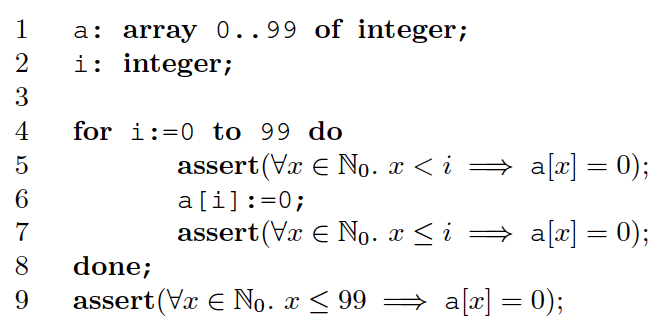
\includegraphics[scale=0.6]{arrayprogex} \\
\\

The postcondition for this program is as follows:
\begin{equation}
\begin{split}
(&\forall{x \in \mathbb{N}} . x<i \implies a[x] = 0)  \\
	&\land a' = a\{i \leftarrow 0\} \\
	&\implies (\forall{x \in \mathbb{N}} . x \leq i \implies a'[x] = 0) 
\end{split}
\end{equation}

Here $a$ and $a'$ represent the array before and after the execution of the program respectively.
Given the pre/post conditions, we can ask for the correctness of the program. As this program is correct, it will satisfy the post-condition. If the program was not correct, then with the help of Rosette we can find out the cause of error and localize the fault. \\
\hcmt {Do I need to write an example of faulty program and show how we want tol get the fault localized (for demonstration purposes)?}
\\
Usually while writing the programs involving arrays, we might make an error while accessing the arrays. This is exactly what we will be focussing on while synthesizing. We shall assume that the error is only on the accessing operation, and with the help of Rosette we will try to fix that.\\\\

{\bf Methodology:}
\begin{enumerate}
	\item  Describing a language which can be used to specify the array manipulating programs with the pre/post conditions and loop invariants \\
	\item Develop an interpreter for this language using Rosette which will help in converting the problem of performing the following analysis of a restricted class of array manipulating programs into instances of SMT array logic internally.
	\begin{itemize}
		\item Verifying an array manipulating program against its specification given as pre-post conditions and loop invariants (for program with loops).
		\item Localizing the location of a bug when verification fails.
		\item Synthesizing a fix for the bug when there exists a fix within a restricted class of possible fixes.\\
		In this project we will focus on the bugs due to array access operations.
	\end{itemize}
	
	\item Implementation of our method within the Rosette-Racket solver-aided programming tool/language framework.\
	
	\item Experiment our implementation on a targeted class of benchmark examples.
\end{enumerate}

\section {Approach}
We will firstly define a basic language which only deals with arrays of integers and provides basic functionalities like accessing and storing in an array. Then we will embed this language with basic programming constructs for arrays in Racket/Rosette.\\
\\
Rosette provides us with various tool to verify, debug and synthesize once we write the interpreter in it. We will then explore how we can automate this process and auto fix the bugs related to array accessing.
\\
\\
We will show with examples how we can use this for debugging and synthesis in such programs.\\
\\
We also plan to create a seperate GUI application which can provide an easy to use interface to the user to get these functionalities. 


\section{Expected Results}
We expect to have a system which can take simple array programs and help the user with verification, debugging and synthesis provided they give either pre/post conditions along with the loop invariants.
\\
Almost all the programs use arrays in one way or another, but most of the useful programs involving arrays also have loops. At least for now, our plan is not to indulge with loops. We might consider the loops if we are successful in the first phase of our project. 


\begin{thebibliography}{unsrt}
	
	\bibitem{rosette_paper}
	E. Torlak and R. Bodik. Growing solver-aided languages with Rosette. In Onward!, 2013.
	
	\bibitem{bugassist}
	Manu Jose and Rupak Majumdar, Cause Clue Clauses: Error Localization Using Maximum Satisfiablity, ACM SIGPLAN conference on Programming Language Design and Implementation (PLDI), June 2011, San Jose, California, USA.
	
\end{thebibliography}


\end{document}